\begin{frame}{Robust nonrandom connectivity patterns}
  % 
  \begin{columns}
    % 
    \begin{column}{.45\textwidth}
      \minipage[c][0.75\textheight][s]{\columnwidth}
      
      \begin{figure}
        \centering
        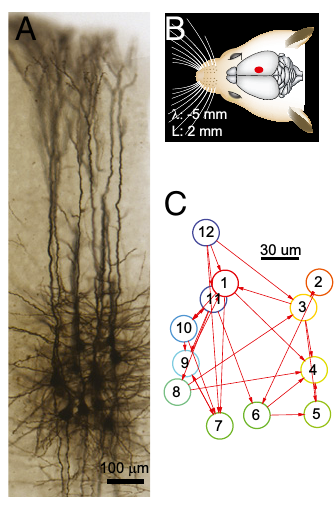
\includegraphics[width=\textwidth]{%
          figures/Perin2011_Fig1ABC.png} %
      \end{figure}
      

      
      \endminipage      
    \end{column}
    % 
    \begin{column}{.55\textwidth}


      \vspace{-0.2cm}
      
      \begin{figure}
        \centering
        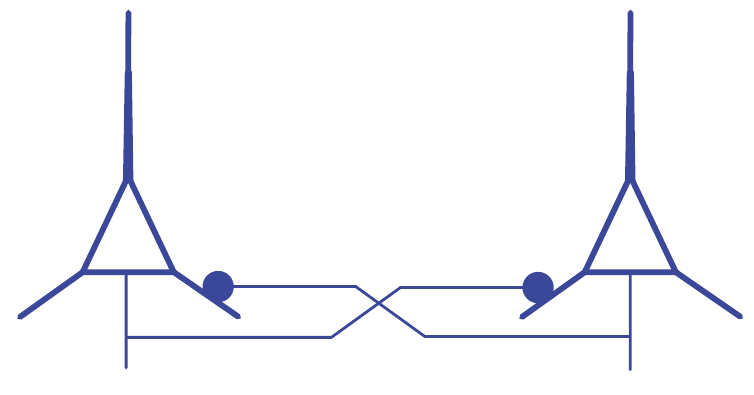
\includegraphics[width=0.525\textwidth]{%
          figures/two_neuron.png} %
      \end{figure}

      \vfill
      

      \begin{figure}
        \centering
        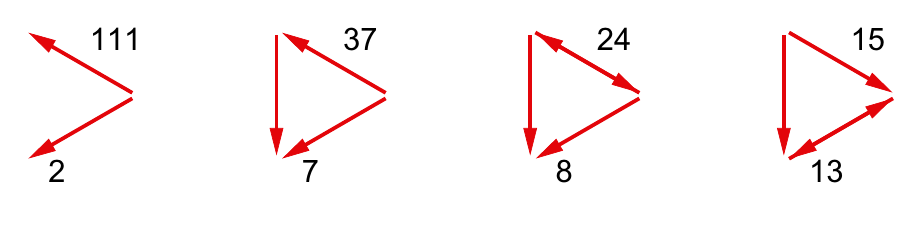
\includegraphics[width=\textwidth]{%
        figures/Perin2011_FigS2_custom.png} %
      \end{figure}

      \vfill
      

      \begin{figure}
        \centering
        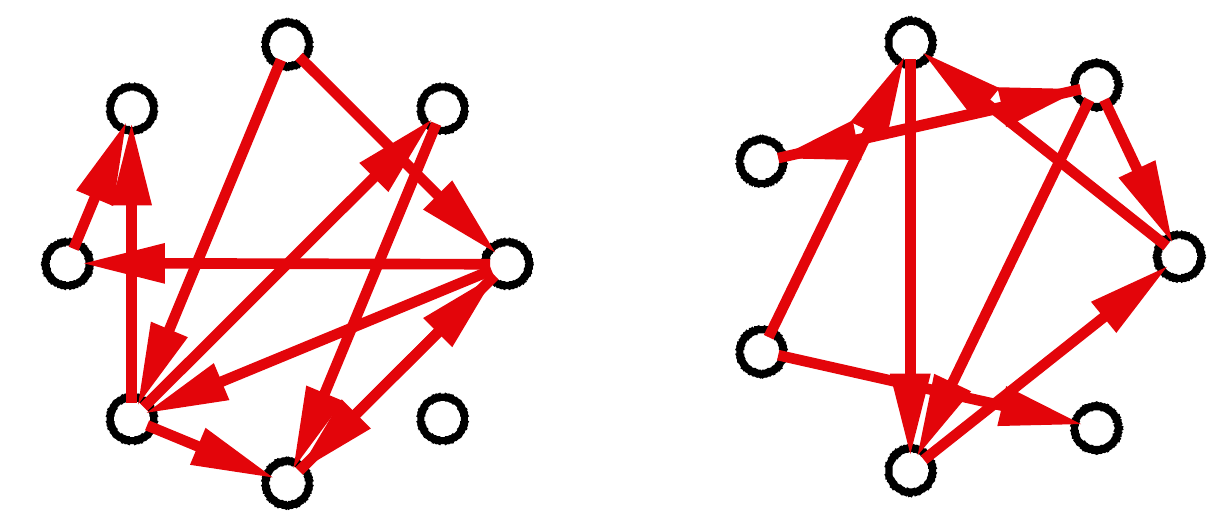
\includegraphics[width=0.7\textwidth]{%
          figures/clust_all.png} %
      \end{figure}
      
      \vfill

      
    \end{column}
  \end{columns}

  \source{\cite{Perin2011, Song2005, Markram1997, Miner2016, Gal2017,
      Vegue2017}}

  \pnote{
    
    These nonrandom structures are well established and have been reported both, 
    
  }
  
\end{frame}




\begin{frame}{Overrepresentation of reciprocal connections}

  
  \begin{figure}
    \centering
    \includegraphics<1>[height=0.78\textheight]{%
      figures/Song2005_Fig2.png} %    
  \end{figure}
  
  \source{\cite{Song2005}}
  
\end{frame}



\begin{frame}{Overrepresentation of reciprocal connections}
  
  \begin{figure}
    \centering
    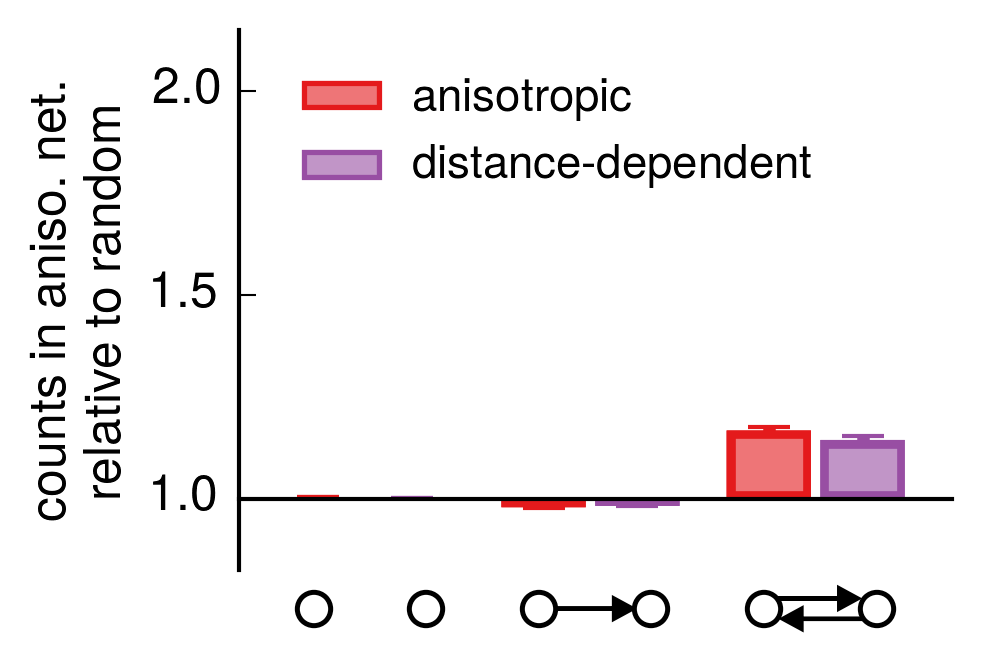
\includegraphics[width=0.78\textwidth]{%
      /home/fh/sci/lab/aniso_netw/ploscb_18/fig/slides/fig3A_2n_rel_rand.png}\hspace{0.9cm}
  \end{figure}
  
\end{frame}




\begin{frame}{Reciprocity -- Distance-dependent?}

  \begin{figure}
    \centering
    \includegraphics<1>[width=\textwidth]{%
      /home/fh/sci/lab/aniso_netw/ploscb_18/fig/slides/fig3C_2n_dstprf_wfit.png} %
    \includegraphics<2->[width=\textwidth]{%
      /home/fh/sci/lab/aniso_netw/ploscb_18/fig/slides/fig3C_2n_dstprf_wfit_data.png} %
  \end{figure}

  \vspace{-0.4cm}

  \only<1-4>{\begin{figure}
    \centering
    \includegraphics<1-2>[width=\textwidth]{%
      /home/fh/sci/lab/aniso_netw/ploscb_18/fig/slides/fig3D_recip_dist.png}
    \includegraphics<3>[width=\textwidth]{%
      /home/fh/sci/lab/aniso_netw/ploscb_18/fig/slides/fig3D_recip_dist_data.png}
    \includegraphics<4>[width=\textwidth]{%
      /home/fh/sci/lab/aniso_netw/ploscb_18/fig/slides/fig3D_recip_dist_data_exp.png}

  \end{figure}}


    \only<5-6>{
    \begin{center}  
    % 
    \minipage[c][0.393\textheight][s]{0.8\textwidth}

    \vspace{0.6cm}
    
    {\large Other sources for the overrepresentation of bidirectional connections?}
    \vfill
    \onslide<6>
    \begin{arrowlist}
      \item {\large Hoffmann, FZ and Triesch, J (2017). Nonrandom
Network Connectivity Comes in Pairs. \textcolor{gray}{\textit{Network Neuroscience}}}
\end{arrowlist}

     \vspace{0.4cm}

     \endminipage
   \end{center}
  }

  
\end{frame}



